% =====================================================================
%  §7. Нелинейный МНК: целевая функция, Левенберг–Марквардт, мультистарт
%
%  ЖАНР (STYLE.md): учебная литература. Ни путей, ни имён программ, ни
%  номеров гипотез. Прослеживаемость — ключи \srckey{7.x} и приложение.
%
%  Содержательная основа: BRIEF_FOR_D_teaching_ladder.md §8; SYNTHESIS.md.
% =====================================================================
\section{Нелинейный МНК: целевая функция, алгоритм, мультистарт}
\label{sec:nonlinear-fit}
\markboth{§\thesection. Нелинейный МНК}{}

Опорная модель курса (§6) содержит десяток параметров: геометрию, коэффициенты потерь, показатель
рассеяния, амплитуду и фазу просачивания, офсет угла. Ни один из них не входит в наблюдаемую
$U(\theta,\nu)$ линейно~--- диаметр стоит внутри логарифмов и рядов формулы Бланко (§2), показатель
рассеяния~--- в показателе степени (§3). Замкнутой формулы решения, какая была в §4, для такой
модели не существует. Этот параграф вводит инструментарий, без которого не обойтись при переходе
от линейной задачи к настоящей: каждое новое понятие появляется здесь как ответ на конкретную
неприятность, которая возникает, как только исчезает линейность.

\begin{tcolorbox}[enhanced,colback=cPanel,colframe=cGrid,boxrule=0.8pt,arc=2pt,
                  title={\bfseries\color{cAccent} Пререквизиты},coltitle=cAccent,
                  attach boxed title to top left={xshift=6pt,yshift=-2pt},
                  boxed title style={colback=cPanel,boxrule=0pt,arc=0pt},top=10pt]
\textbf{Нужно знать:} §4 (МНК, ковариация, веса) и §5 (корреляция, эллипс, обусловленность) как
образец того, что удаётся сделать в замкнутой форме; §6 (полный список параметров опорной
модели).\\[0.3em]
\textbf{Знать НЕ нужно:} вывод алгоритма Левенберга--Марквардта из первых принципов~--- здесь он
изложен на уровне интуиции, достаточном, чтобы понимать, что и почему может пойти не так.
\end{tcolorbox}

% ---------------------------------------------------------------------
\subsection{Целевая функция}
\label{subsec:objective}

За неимением замкнутого решения задача ставится явно: подобрать вектор параметров~$\mathbf{p}$,
минимизирующий взвешенную сумму квадратов невязок между моделью и измерением по всем углам и
частотам сразу:
\begin{equation}
  \mathbf{p}^\star=\argmin_{\mathbf{p}}\ \chi^2(\mathbf{p})
  =\argmin_{\mathbf{p}}\sum_{i}w_i\big[y_i-f(\mathbf{p};\theta_i,\nu_i)\big]^2 .
  \label{eq:objective}
\end{equation}
Формально это то же самое выражение, что и в §4~--- сумма взвешенных квадратов,~--- но $f$ теперь
нелинейна по~$\mathbf{p}$, и потому нормальные уравнения~\eqref{eq:normal-eq} перестают быть
линейной системой: производная $\partial\chi^2/\partial\mathbf{p}=0$ сама содержит~$\mathbf{p}$
нелинейно.

% ---------------------------------------------------------------------
\subsection{Веса амплитуды и фазы}
\label{subsec:weights-amp-phase}

Урок §\ref{subsec:weights} о весах здесь возвращается в усложнённом виде. Модель предсказывает не
только амплитуду сигнала, но и его фазу (§0, §1)~--- а амплитуда и фаза измеряются в разных
единицах и имеют разный динамический диапазон. Без отдельных весов для каждой из них одна
компонента невязки статистически подавляет другую~--- тот же эффект, что заглушение тени ярким
сигналом в §4, только теперь между двумя разнородными наблюдаемыми, а не между разными участками
одной и той же кривой. Решение~--- те же принципы, что в §4: взвешивать так, чтобы относительный
вклад каждой компоненты отражал её информативность, а не её случайный численный масштаб.

% ---------------------------------------------------------------------
\subsection{Маска динамического диапазона}
\label{subsec:mask}

\begin{warning}[: не весь диапазон данных одинаково надёжен]
В самой глубокой тени (углы, близкие к $90^\circ$) сигнал приближается к шумовому полу прибора:
там измеряется в основном шум, а не физика просачивания. Включение таких точек в подгонку с полным
весом добавляет в целевую функцию шум, который модель пытается <<объяснить>>, портя оценку
параметров, отвечающих именно за эту область.
\end{warning}

\noindent
Стандартное решение~--- \term{маска}: точки с отношением сигнал/шум ниже порога исключаются из
суммы~\eqref{eq:objective} или получают нулевой вес. Естественный вопрос: не превращается ли
результат затем в артефакт самой маски~--- не выбрасываем ли мы заодно и содержательный сигнал?

\begin{example}[: проверка того, что маска не создаёт эффект, а очищает его]\srckey{7.1}
Введение маски не ослабило, а \emph{усилило} свидетельство в пользу просачивания: улучшение
информационного критерия при добавлении явного просачивания выросло с $\dAIC\approx-533$ без
маски до $\dAIC\approx-657$ с ней. Если бы эффект был артефактом шума, маскирование шума должно
было бы его ослабить; произошло обратное~--- значит эффект не является порождением немаскированных
шумовых точек.
\end{example}

% ---------------------------------------------------------------------
\subsection{Алгоритм: гибрид спуска и метода Гаусса--Ньютона}
\label{subsec:lm}

\begin{intuition}
Вдали от минимума градиентный спуск надёжен, но медлителен: он делает маленькие осторожные шаги
вниз по склону. Вблизи минимума, где целевая функция похожа на параболу, метод
Гаусса--Ньютона сходится почти мгновенно, но вдали от минимума может <<перелететь>> или разойтись,
потому что опирается на локальную квадратичную аппроксимацию, верную только вблизи решения.
\term{Алгоритм Левенберга--Марквардта} плавно переключается между двумя стратегиями: параметр
затухания делает шаг похожим на осторожный градиентный спуск, когда прогресс плохой, и на быстрый
шаг Гаусса--Ньютона, когда прогресс хороший. Это стандартный рабочий инструмент нелинейного МНК
--- не единственный, но самый привычный выбор по умолчанию для задач такого размера.
\end{intuition}

% ---------------------------------------------------------------------
\begin{figure}[t]
  \centering
  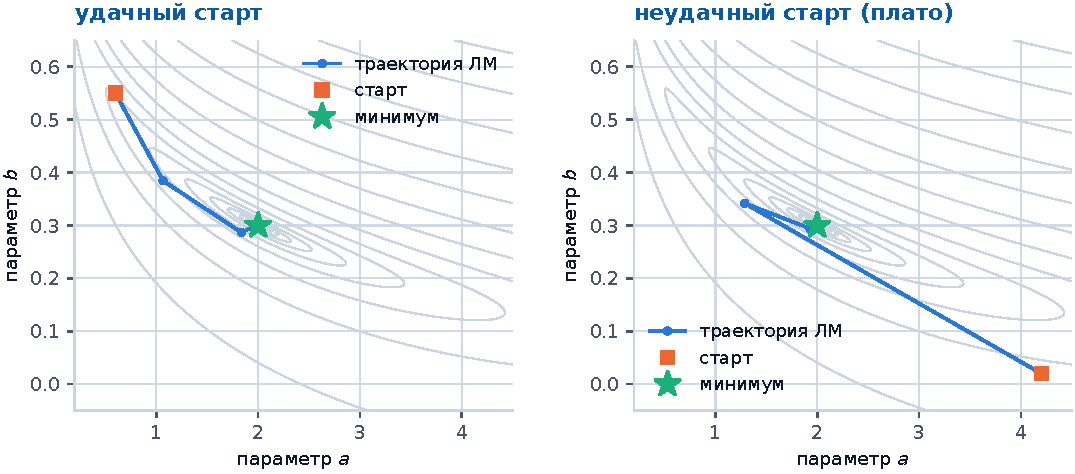
\includegraphics[width=0.86\linewidth]{figures/fig07_lm_trajectory.pdf}
  \caption{Иллюстрация алгоритма на учебной модельной задаче (не данные проекта): траектория
  Левенберга--Марквардта на линиях уровня целевой функции при удачном (сходится быстро) и
  неудачном (стартует в области, откуда путь к глобальному минимуму идёт через плоское плато)
  начальном приближении. Показана механика алгоритма, а не какой-либо из параметров опорной
  модели курса.}
  \label{fig:lm-trajectory}
\end{figure}

% ---------------------------------------------------------------------
\subsection{Начальное приближение перестаёт быть формальностью}
\label{subsec:init}

В линейной задаче §4 минимум был один, и стартовая точка не имела значения вообще~--- любое
решение линейной системы даёт один и тот же ответ. У нелинейной целевой функции может быть
\textbf{несколько локальных минимумов}, и алгоритм из §\ref{subsec:lm} находит ближайший к
стартовой точке, а вовсе не обязательно глобальный. Начальное приближение перестаёт быть
технической деталью и становится содержательным решением.

\begin{intuition}[: откуда берётся хороший старт почти бесплатно]
Гармонический разбор §4~--- решение линейной системы без итераций~--- сам по себе даёт оценки
офсета угла, амплитуды просачивания и относительной фазы каналов. Это не полная нелинейная
модель, но она даёт разумное первое приближение для соответствующих параметров нелинейной модели
почти без дополнительных затрат: \term{тёплый старт} из линейного разбора~--- стандартная практика,
которой стоит пользоваться всегда, когда она доступна.
\end{intuition}

% ---------------------------------------------------------------------
\subsection{Мультистарт и области притяжения}
\label{subsec:multistart}

\begin{warning}[: тёплый старт один — не гарантия]
Даже хороший тёплый старт не гарантирует сходимости к глобальному минимуму: у сложной модели
может быть несколько содержательно разных \term{областей притяжения}~--- множеств стартовых точек,
из которых алгоритм сходится к одному и тому же локальному решению,~--- и заранее не известно,
в какой из них попадёт конкретный старт.
\end{warning}

\begin{example}[: сколько стартов нужно на практике]\srckey{7.2}
На опорной модели курса из $21$ случайно выбранной стартовой точки в разных запусках получалось
от $3$ до $20$ различных областей притяжения (число зависело от конкретного набора данных и
параметризации), а доля стартов, попадающих в область глобального минимума, составила лишь
\textbf{$22{,}2\,\%$}. Решения из разных областей притяжения группировались по близости
информационного критерия (в пределах $0{,}5$ единиц $\AIC$), чтобы не считать одно и то же
решение, найденное с разной точностью сходимости, за <<разные>> результаты.
\end{example}

\begin{tcolorbox}[enhanced,colback=cS2!6,colframe=cS2,boxrule=0pt,leftrule=3pt,arc=1pt]
\textbf{История одной ошибки, которую стоит знать любому, кто планирует пользоваться нелинейным
МНК.} Раннее эмпирическое правило гласило: «тёплый старт лучше холодного, одного разумного старта
достаточно». Это правило пришлось \emph{отменить} после систематической проверки на сетке
стартов~--- выяснилось, что в глобальную область притяжения попадают лишь $22{,}2\,\%$ запусков, а
значит, единственный, пусть и разумный, старт даёт лишь вероятностный, а не гарантированный
результат.
\end{tcolorbox}

\begin{warning}[: конкретная цена одного старта — реальный отозванный результат]\srckey{7.3}
Значение перекрёстного члена $|\varepsilon_{\rm cross}|=0{,}0345$, ранее опубликованное по
результату одного старта, оказалось решением из \textbf{четвёртого} по качеству бассейна из
одиннадцати найденных~--- хуже глобального минимума на $192{,}5$ единиц информационного
критерия (шкала~--- §\ref{subsec:pay-principle}, «категорически хуже»). Число было отозвано,
как только сетка стартов вскрыла его происхождение. Здесь оно приводится единственный раз и
исключительно как иллюстрация того, к чему приводит доверие одному старту без проверки сеткой:
использовать его как физический результат~--- нельзя (полный список причин~--- в служебном
приложении курса).
\end{warning}

% ---------------------------------------------------------------------
\begin{figure}[t]
  \centering
  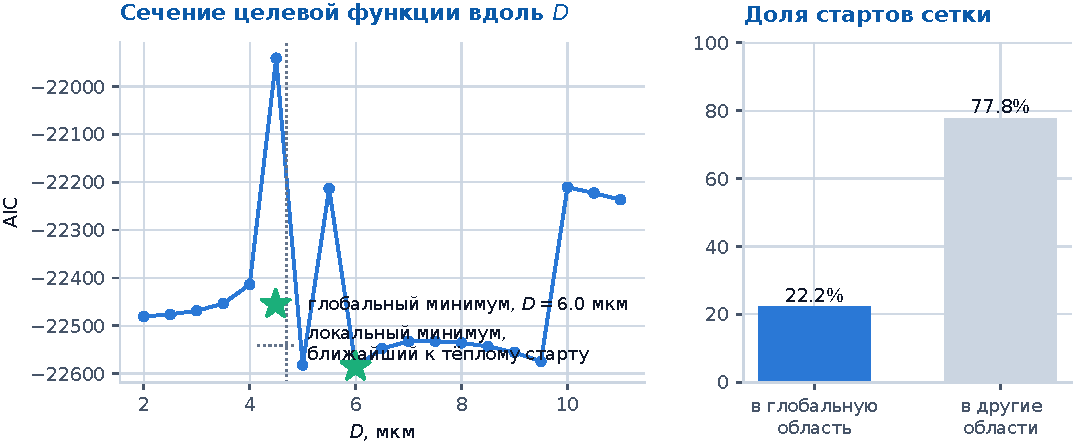
\includegraphics[width=\linewidth]{figures/fig07_basins.pdf}
  \caption{Слева: сечение целевой функции (информационный критерий) вдоль одного из параметров
  геометрии при фиксированных остальных~--- реальный расчёт, несколько локальных минимумов
  видны непосредственно на кривой; глобальный минимум отмечен отдельно, и он не совпадает с
  минимумом, ближайшим к границе физически правдоподобных значений. Справа: доля стартов,
  попадающих в область глобального минимума, по результатам сеточной проверки
  (§\ref{subsec:multistart}).}
  \label{fig:basins}
\end{figure}

% ---------------------------------------------------------------------
\subsection{Фиксация параметров при вырождении}
\label{subsec:pinning}

Когда два параметра почти неразличимы данными (§5 показал этот механизм в линейной задаче;
здесь он вернётся в §9 в полном объёме), свободная подгонка обоих~--- не консервативный, а
бессмысленный выбор: алгоритм найдёт какую-то комбинацию, устраивающую данные, но отчёты об
отдельных значениях будут вводить в заблуждение. Практический выход~--- \term{зафиксировать}
(«приколотить») один из вырожденных параметров на независимо обоснованном значении и подгонять
только второй. Так эффективный диаметр в опорной модели курса фиксируется не потому, что его
не пытались подгонять свободно, а потому, что свободная подгонка вместе с просачиванием даёт
не число, а признание собственной неопределённости, замаскированное под число (полный разбор~---
§9).

% ---------------------------------------------------------------------
\subsection{Ковариация без замкнутой формулы: бутстрап}
\label{subsec:bootstrap}

В линейной задаче §4 ковариация оценок была точной формулой. Для нелинейной модели стандартная
практика~--- приближённая ковариация вблизи минимума (обсуждается в §9) либо
\term{бутстрап}~--- многократное повторение подгонки на случайно пересемплированных версиях
данных, дающее эмпирическое распределение оценки.

\begin{warning}[: бутстрап требует независимости, а её нужно проверять, а не предполагать]\srckey{7.4}
Ресемплирование по отдельным точкам корректно только тогда, когда точки данных статистически
независимы. Пересемплирование \emph{по частотным отсчётам} на наших данных занижает ошибку в
$3{,}5$--$18{,}9$~раз, потому что соседние частотные точки коррелированы (одна и та же
физическая реализация шума и общий частотный профиль прибора размазаны по соседним отсчётам).
Ресемплирование должно происходить по единицам, которые \emph{действительно} независимы~---
например, по отдельным независимым измерениям, а не по каждой точке частотной сетки внутри
одного измерения.
\end{warning}

% ---------------------------------------------------------------------
\subsection{Типичные ошибки этого параграфа}

\begin{enumerate}[leftmargin=1.6em,itemsep=0.25em]
  \item Использовать один разумный (пусть и тёплый) старт и принимать результат как окончательный.
        Только сеточная проверка показывает, попал ли алгоритм в глобальную область притяжения
        (§\ref{subsec:multistart}).
  \item Расширять маску динамического диапазона, не проверив, усиливает или ослабляет она искомый
        эффект (§\ref{subsec:mask}) — иначе легко принять артефакт маскирования шума за
        содержательный результат, или наоборот, вычистить реальный эффект вместе с шумом.
  \item Свободно подгонять оба параметра из вырожденной пары «на всякий случай». Результат~---
        число, не несущее информации по отдельности (§\ref{subsec:pinning}, полный разбор~--- §9).
  \item Бутстрапировать по единицам данных, независимость которых не проверена. Соседние
        частотные отсчёты — типичный пример мнимой независимости (§\ref{subsec:bootstrap}).
  \item Забыть, что у Левенберга--Марквардта, как и у любого локального метода, нет встроенной
        гарантии глобальности~--- она появляется только вместе с мультистартом.
\end{enumerate}

\clearpage
